\subsection{Parking Lot Generation}
The ParkingGenerator is implemented as a function that takes a plot and its underlying terrain as input and produces a parking lot as output (see Table~\ref{table:parking}).
This generator in particular is responsible for filling roughly ten percent of the generated cities with parking lots, a percentage based on research conducted in Phoenix,~AZ~\cite{parking_percent}.
\begin{table}[H]
   \centering
   \begin{tabular}{lllll}
     \textbf{Input}                           &               & \textbf{Function}            &               & \textbf{Output}         \\
     \midrule
     \textit{Plot, Terrain}                   & $\rightarrow$ & \textbf{ParkingGenerator}       & $\rightarrow$ & \textit{Parking lot}           \\
     \bottomrule
   \end{tabular}

   \caption{Definition of the ParkingGenerator function which is responsible for generating parking lots.}
   \label{table:parking}
 \end{table}
 \vspace{-0.4cm}

One considered approach for generating parking lots was Esri CityEngine's \cite{Esri}.  % having a hard time finding this source, Anton who found it... plz help me. 
What they use, for at least some of their generation is simply covering areas with textures. This can be seen in their parks and parking lots. 
This was at first considered to be a viable option for the project, only it was found that it offers little alternatives for modification. 

Modification, in this remark, includes the shape of the entire parking lot as well as the size of the individual parking spaces.
As every other generator provides fully scalable content, it would be inconvenient for the ParkingGenerator to be any different.
If it were to make use of quads with a single texture applied to them, it would remove the possibility of scaling the size of the parking spaces within the quad without scaling the quad itself.

The approach instead elected for was an algorithm that generates the parking spaces individually.
This algorithm works by first using a function for approximating the largest rectangle inside any given polygon. 
The reasoning behind this was the group's observation that parking lots seem to have a rectangular shape generally (see Figure~\ref{fig:parkings}).
This shape does of course not apply to every parking lot in the world, however attempting to create parking lots of any size and shape would require a lot more effort, and was therefore deemed out of scope for this project. 
\begin{figure}[H]
  \centering
  \begin{subfigure}[b]{0.56\textwidth}
    \frame{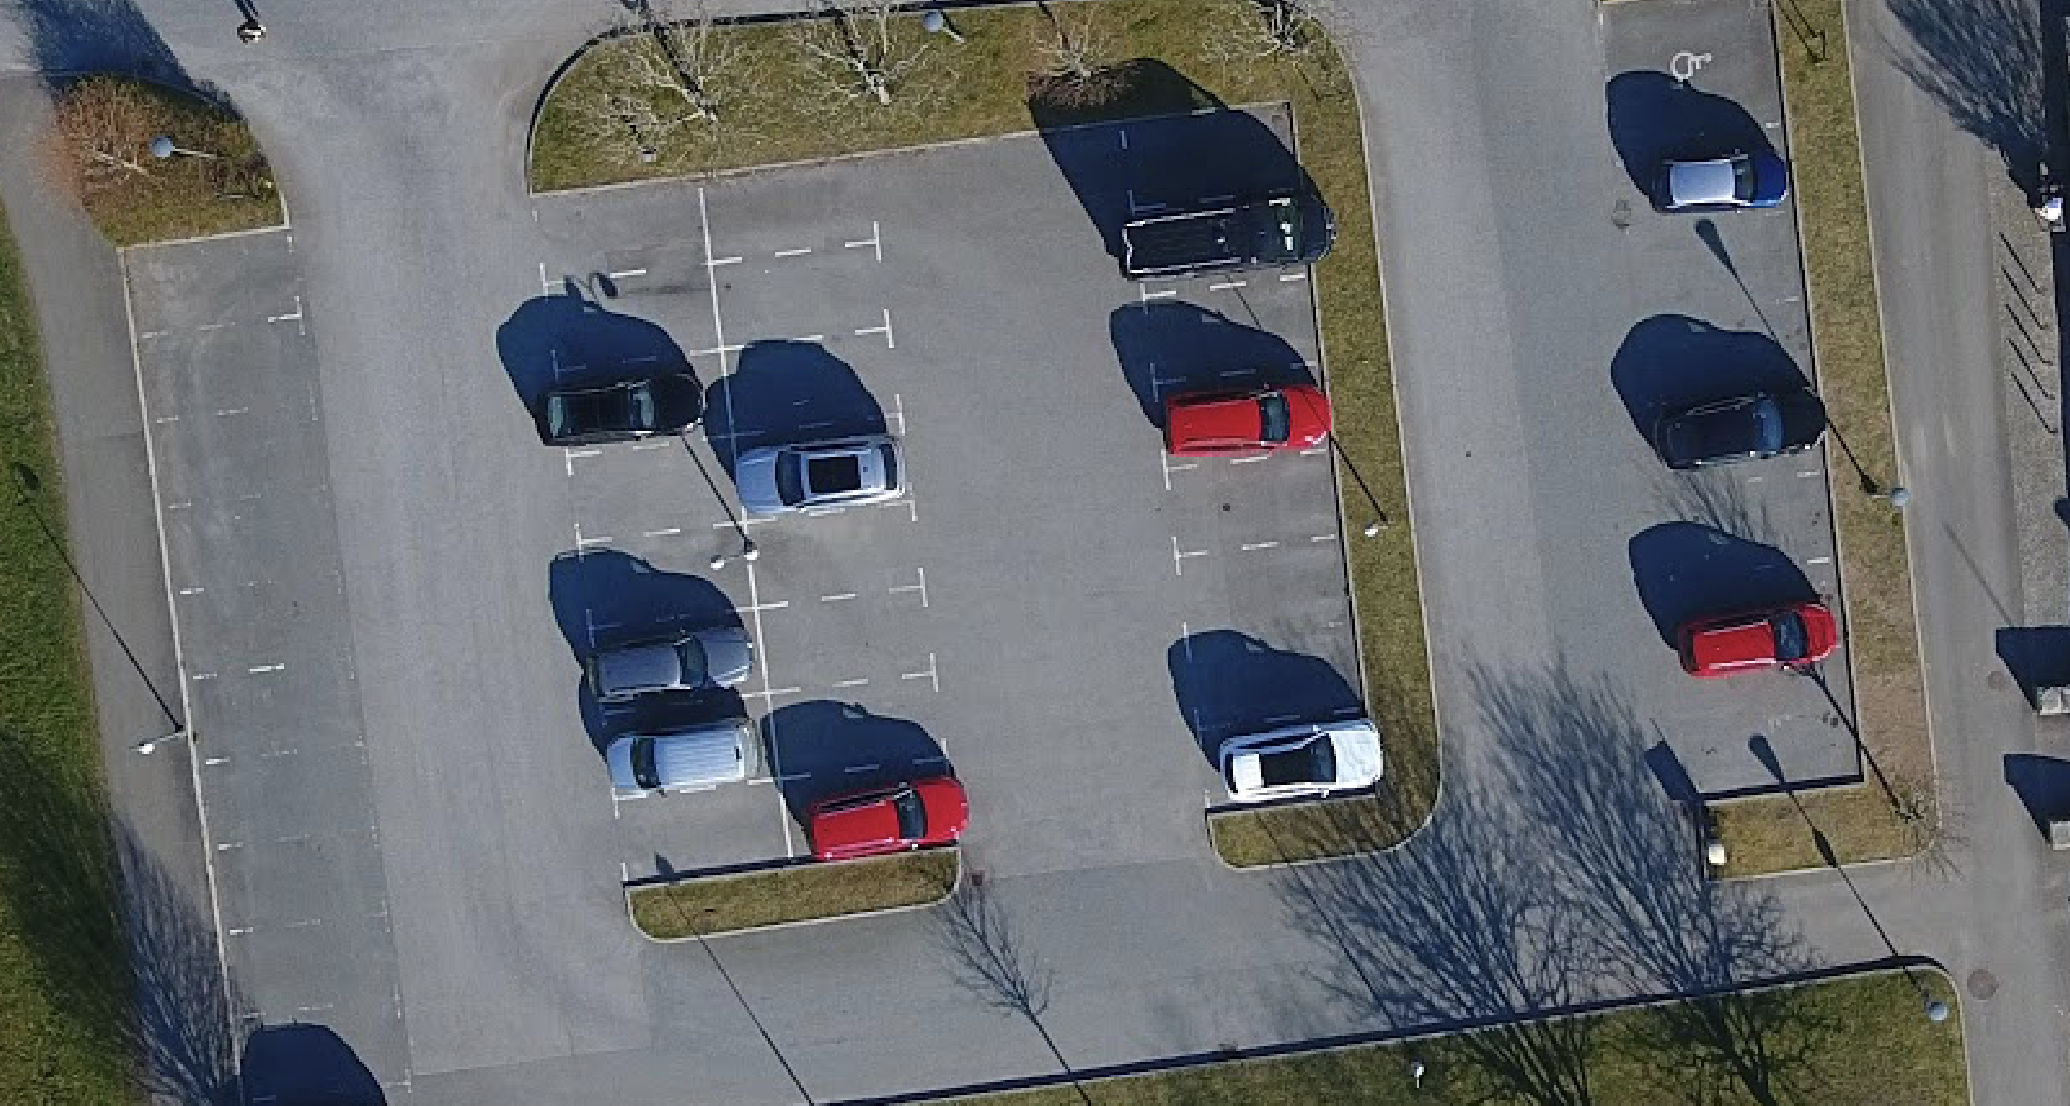
\includegraphics[width=\textwidth]{figure/parking1}}
  \end{subfigure}
  \quad
  \begin{subfigure}[b]{0.395\textwidth}
    \frame{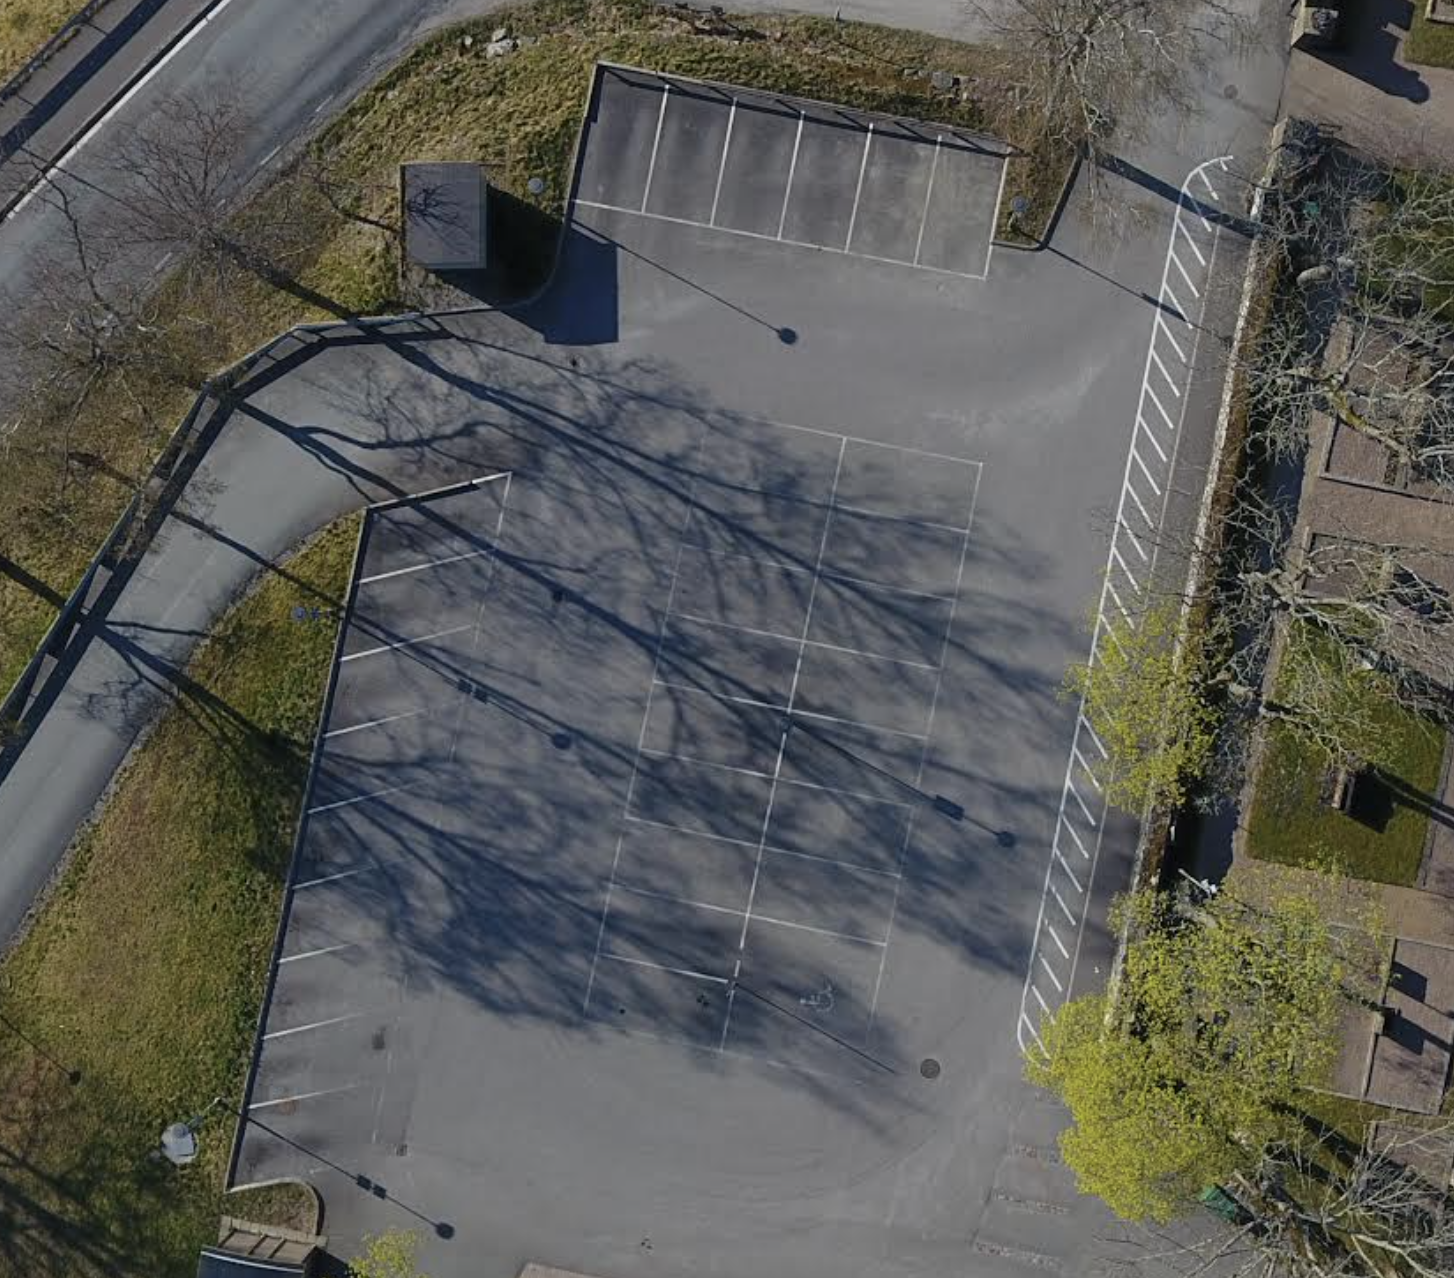
\includegraphics[width=\textwidth]{figure/parking2}}
  \end{subfigure}
  \caption{Two examples of parking lots observed by the project group, showcasing the rectangular shapes mentioned above.}
  \label{fig:parkings}
\end{figure}
Afterward, based on the size of the rectangle, the algorithm would then generate either two or four columns of parking spaces (see Figure~\ref{fig:sizebased}).
\begin{figure}[H]
  \centering
  \begin{subfigure}[b]{0.56\textwidth}
    \frame{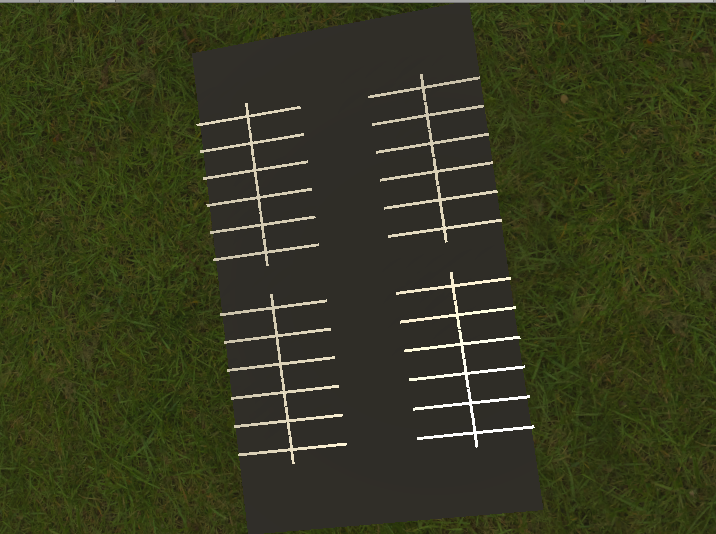
\includegraphics[width=\textwidth]{figure/fourcol}}
    \caption{Large parking lot consisting of four columns.}
  \end{subfigure}
  \quad
  \begin{subfigure}[b]{0.395\textwidth}
    \frame{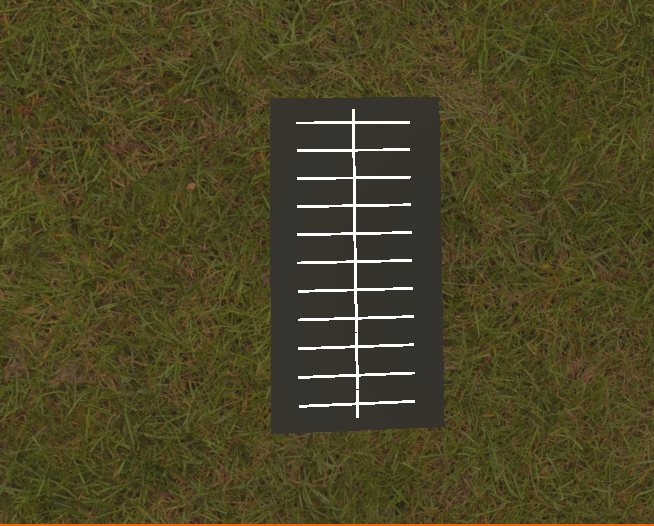
\includegraphics[width=\textwidth]{figure/twocol}}
    \caption{Small parking lot consisting of two columns.}
  \end{subfigure}
    \caption{Two examples of different sized parking lots created by the generator.}
  \label{fig:sizebased}
\end{figure}

